\section{\label{section3}Overview of technique and apparatus}
\subsection{Outline of technique}
The X-ray technique measures the axial (Z) and azimuthal ($\phi$)
position of each photodetector (or MPPC) by scanning individual
photodetector with a well collimated beam of X-ray. The beam is
precisely located in the azimuthal and axial coordinates, and pointed
radially originating from the central axis of MEG (Figure
\ref{fig:photo}).  The collimator projects a thin (1$\times$30~mm, 1.5$\times$50
mrad$^2$) beam on the inner face of cryostat, about 8\% the width of
the MPPC in the narrow dimension, whose motion is controlled by
precise linear and rotation stages. A coordinate of the
MPPC is calculated by orienting the narrow dimension of the beam in
that direction and scanning. The signal from the scintillating light
as a function of X-ray beam position determines the spatial extent of
the MPPC. The spatial resolution as well as exposure time per position
is chosen to balance the desired statistical precision and the time
budget allocated for the calorimeter scan. A test X-ray scan of cubic
(6~mm) LYSO scintillator is shown in figure \ref{fig:beamprofile}.

The X-rays are produced by the decays of \cob source which produces
two X-ray emission lines at 122 keV ($\approx$80\%) and 136 keV
($\approx$10\%).  A commercially produced point source with
activity of 3$\times 10^{10}$ Bq is used. The energy of source is
chosen such that it penetrates the magnetic and calorimetric cryostats
but low enough to interact with liquid Xe within $\approx$3~mm. The light
detected by the MPPCs is produced close to the surface of the
photodetector primarily by photo-absorption, and generates signal of
about 30\% that of a typical 53 MeV photon from \mueg events. Raw
waveform and pulse-height distributions for a given channel
illuminated with and without X-rays show the magnitude of the observed
signal (Figure \ref{fig:pulseheight}).

The precision of the measurement depends on the precision with which
the X-ray coordinates can be determined. 
The apparatus is aligned by means of optical survey so that the X-ray 
motion is coaxial with the COBRA magnet centered in the MEG coordinate system, 
and small variations in the X-ray position are monitored with a laser system 
and a bubble-level. 
We rely on the position information from the motion stages which is corrected
for known angular and linear misalignments. 
An additional cross-check of the X-ray position calculations is performed 
by placing precisely aligned lead absorber strips (30$\times$3~mm$^2$) on the 
front face of LXe cryostat. 
The lead positions are determined with optical
survey and independently with supressed X-ray events (shadow)
in the scanning of the photodetectors.
The agreement between these measurements is used for validaiton of X-ray 
alignment and correction procedures, and serves as the upper limit of the precision 
of the measurement. 

A high precision 3D FARO scan\cite{faro} of the MPPCs is carried out
in an open, unfilled calorimeter at room temperature.  This serves as
a complimentary measurement to the X-ray survey, and a benchmark for
studying the effects of cryogenically cooled calorimeter on the
photodetectors.

\begin{figure}[]
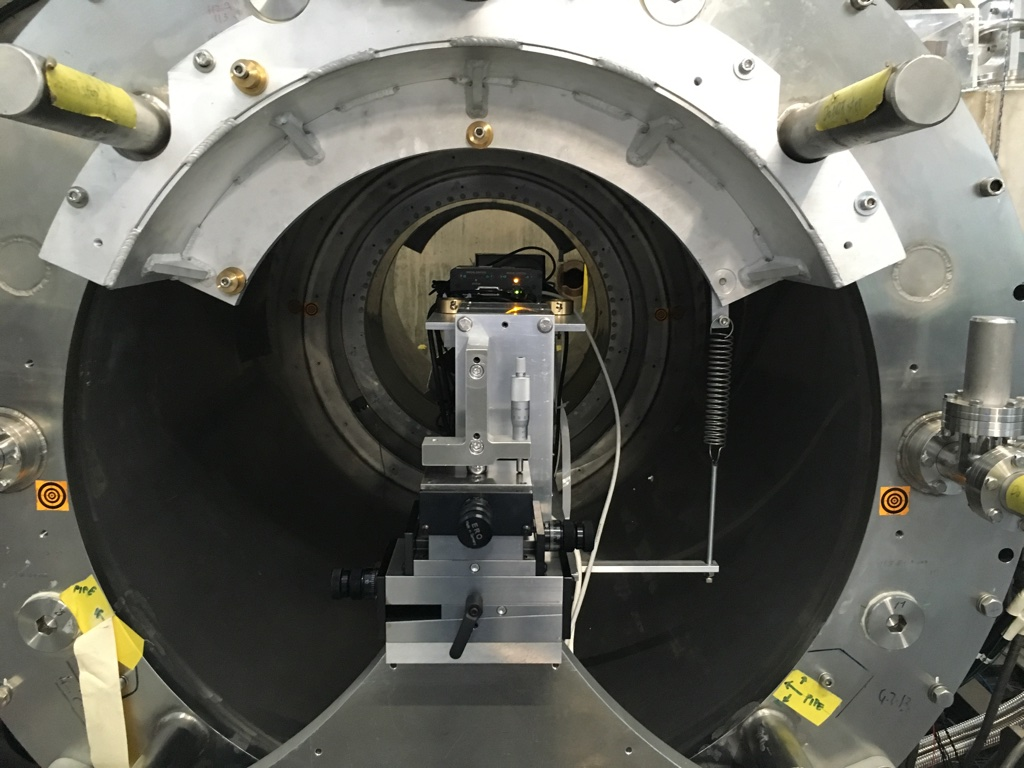
\includegraphics[width=8cm]{plots/photo4}
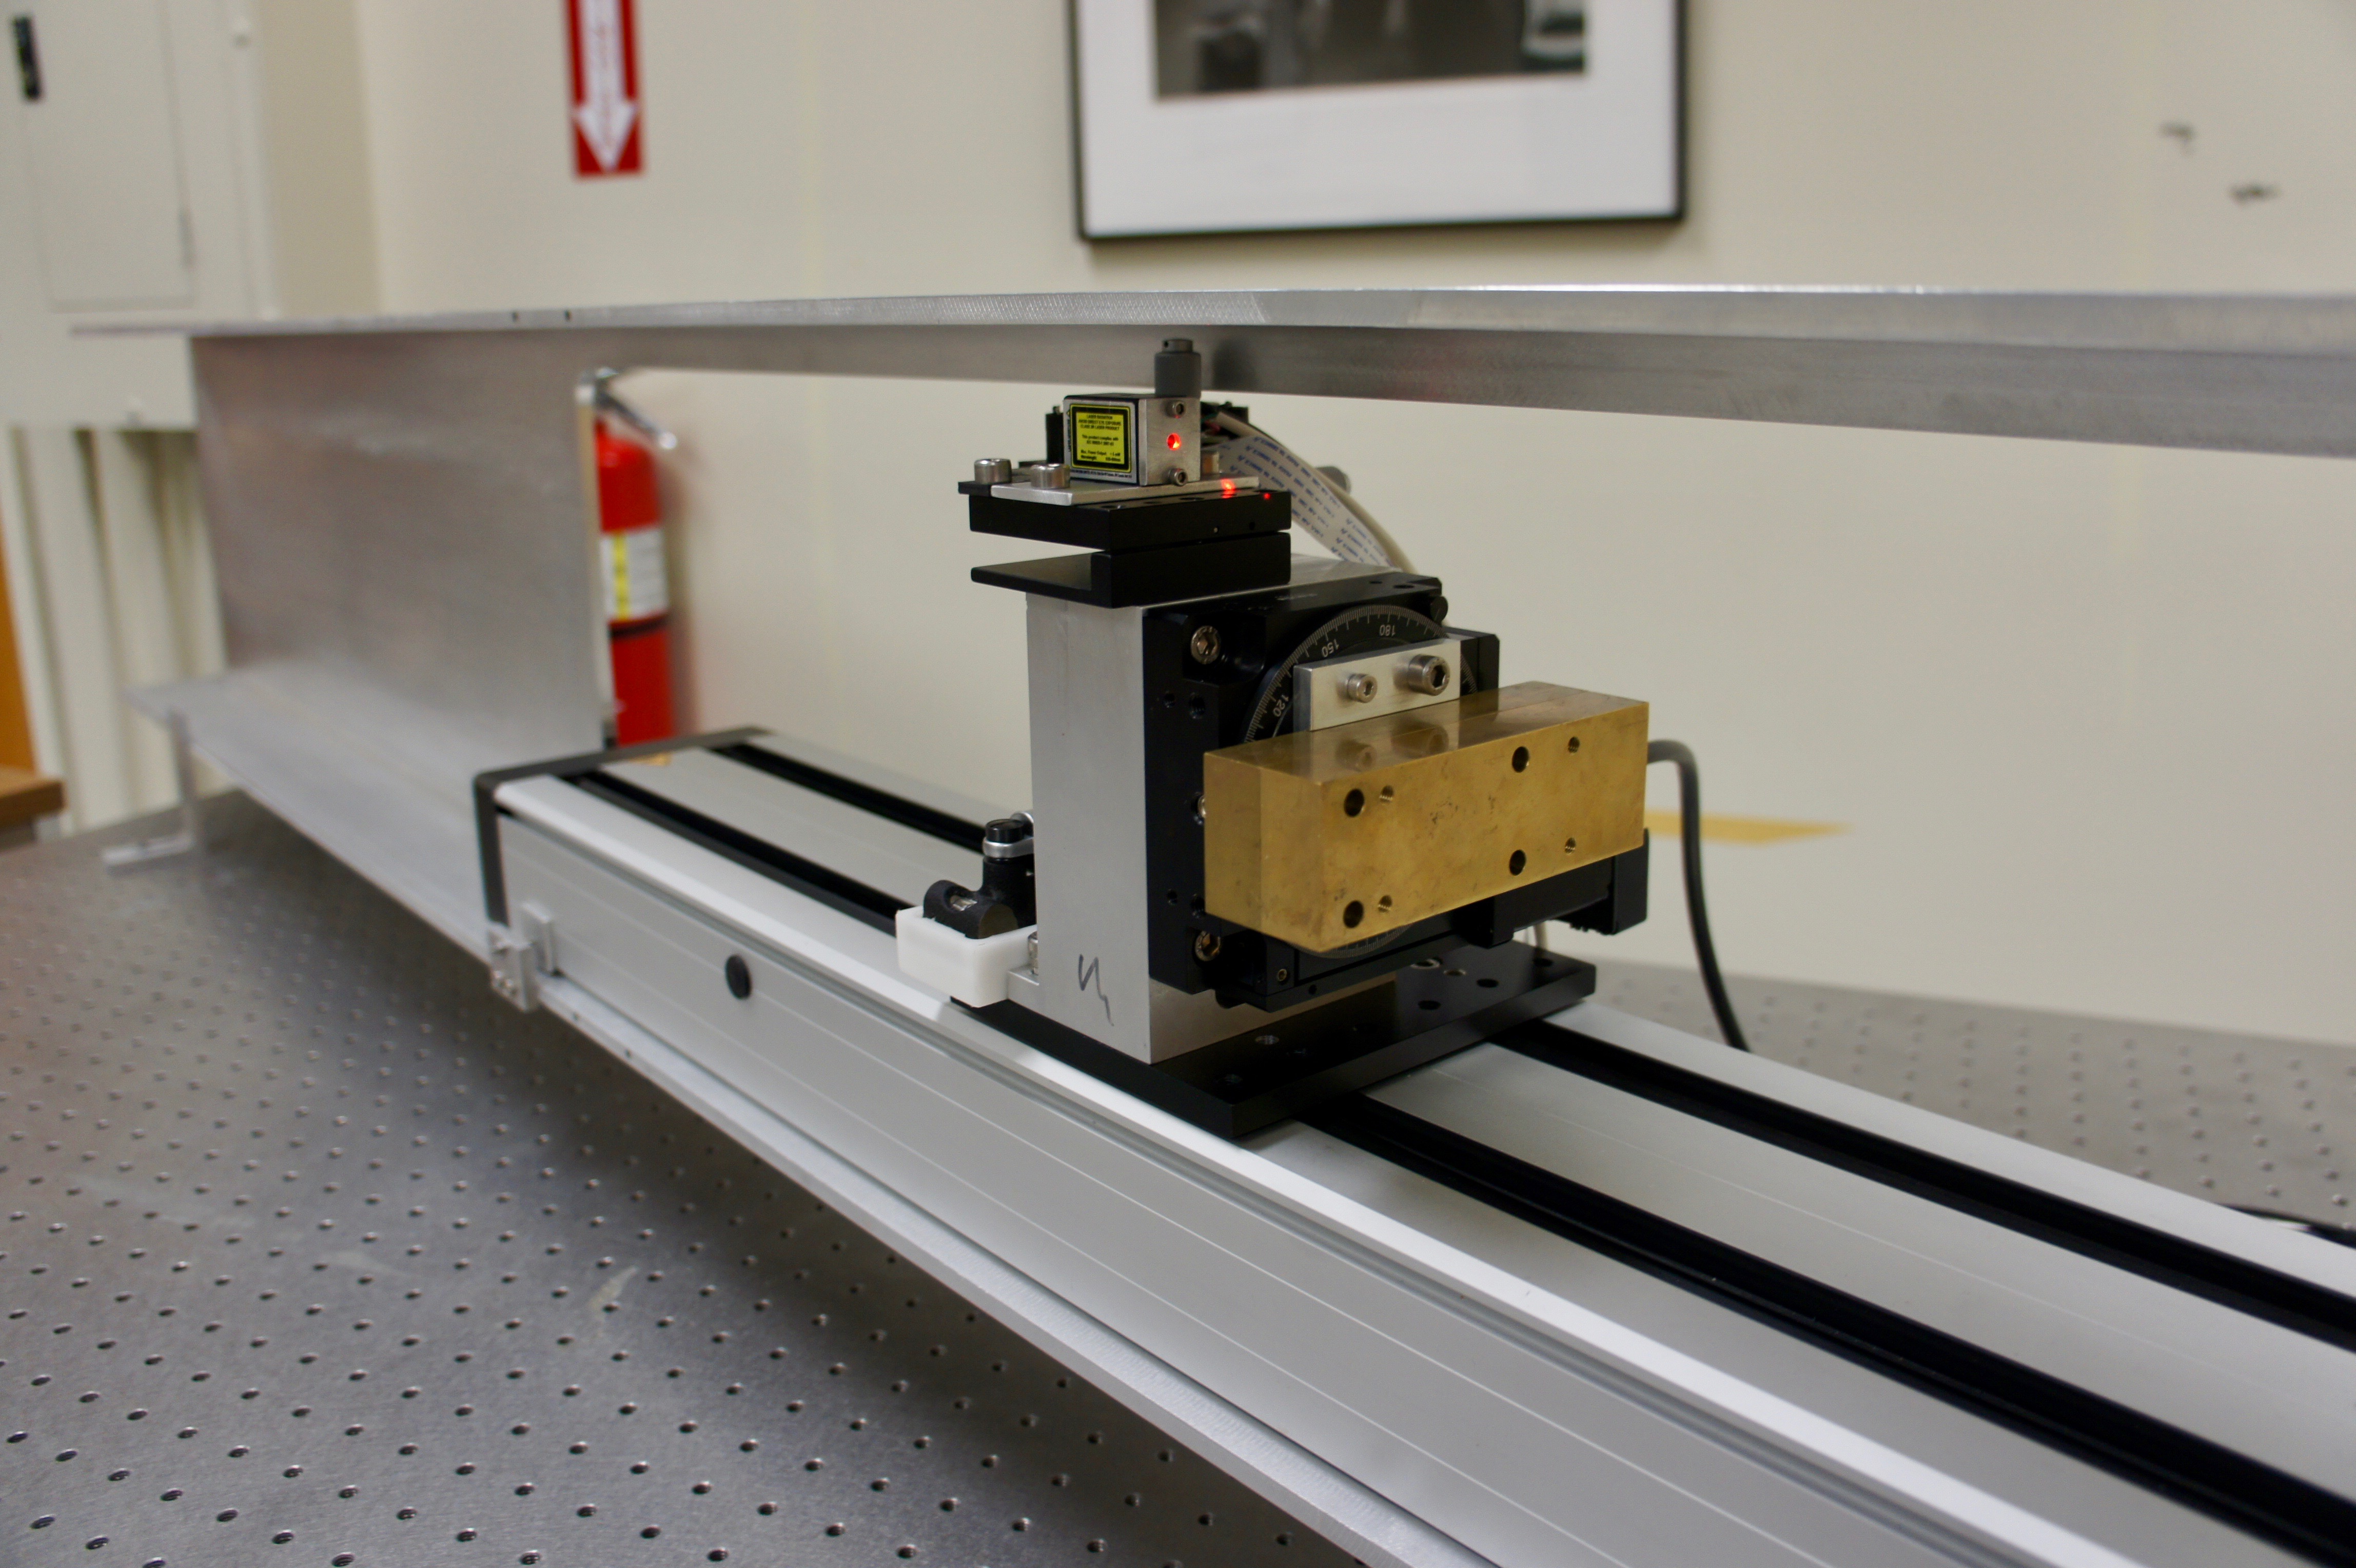
\includegraphics[width=8cm]{plots/photo3}
\caption{X-ray survey apparatus shown mounted inside COBRA magnet
  (left) and outside the experimental area (right).}
\label{fig:photo}
\end{figure}  

\begin{figure}[]
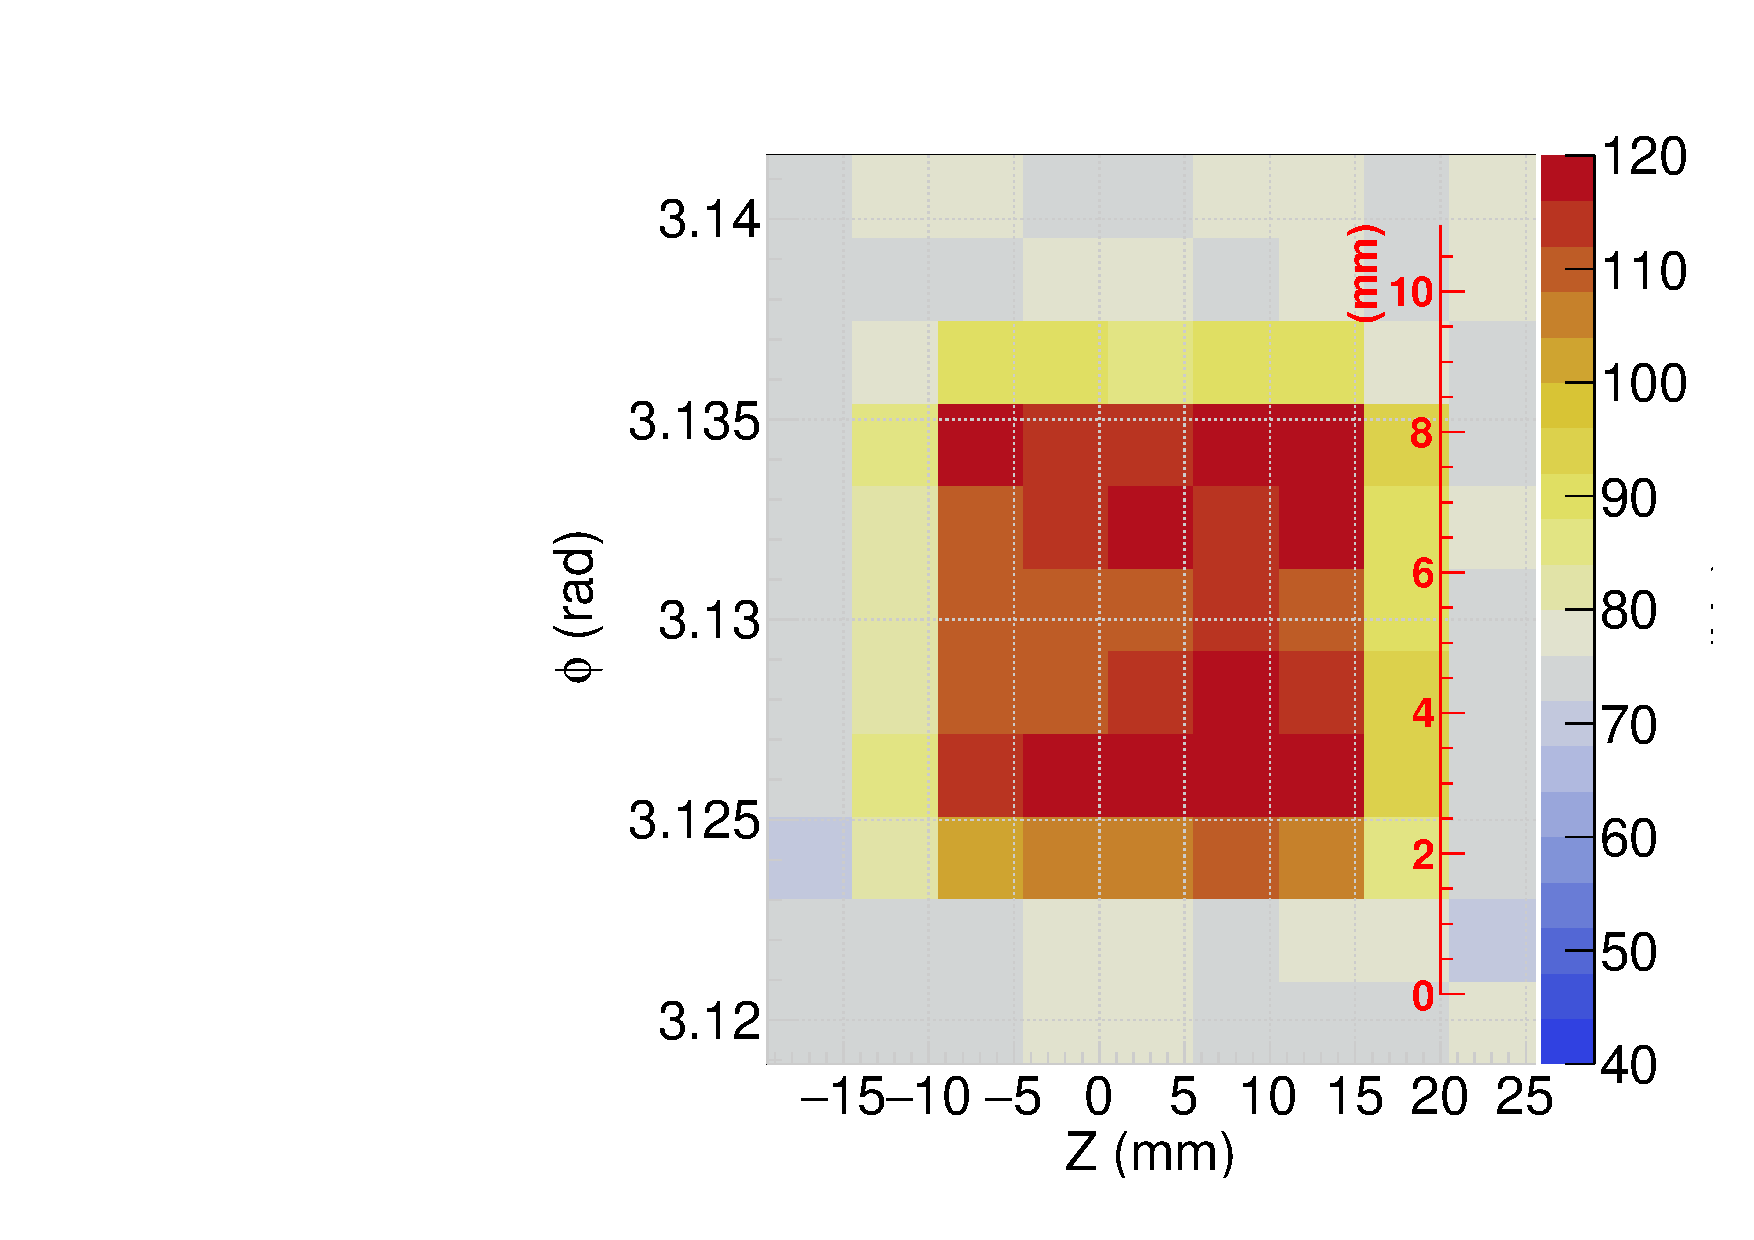
\includegraphics[width=4cm]{plots/xray_lyso.pdf}
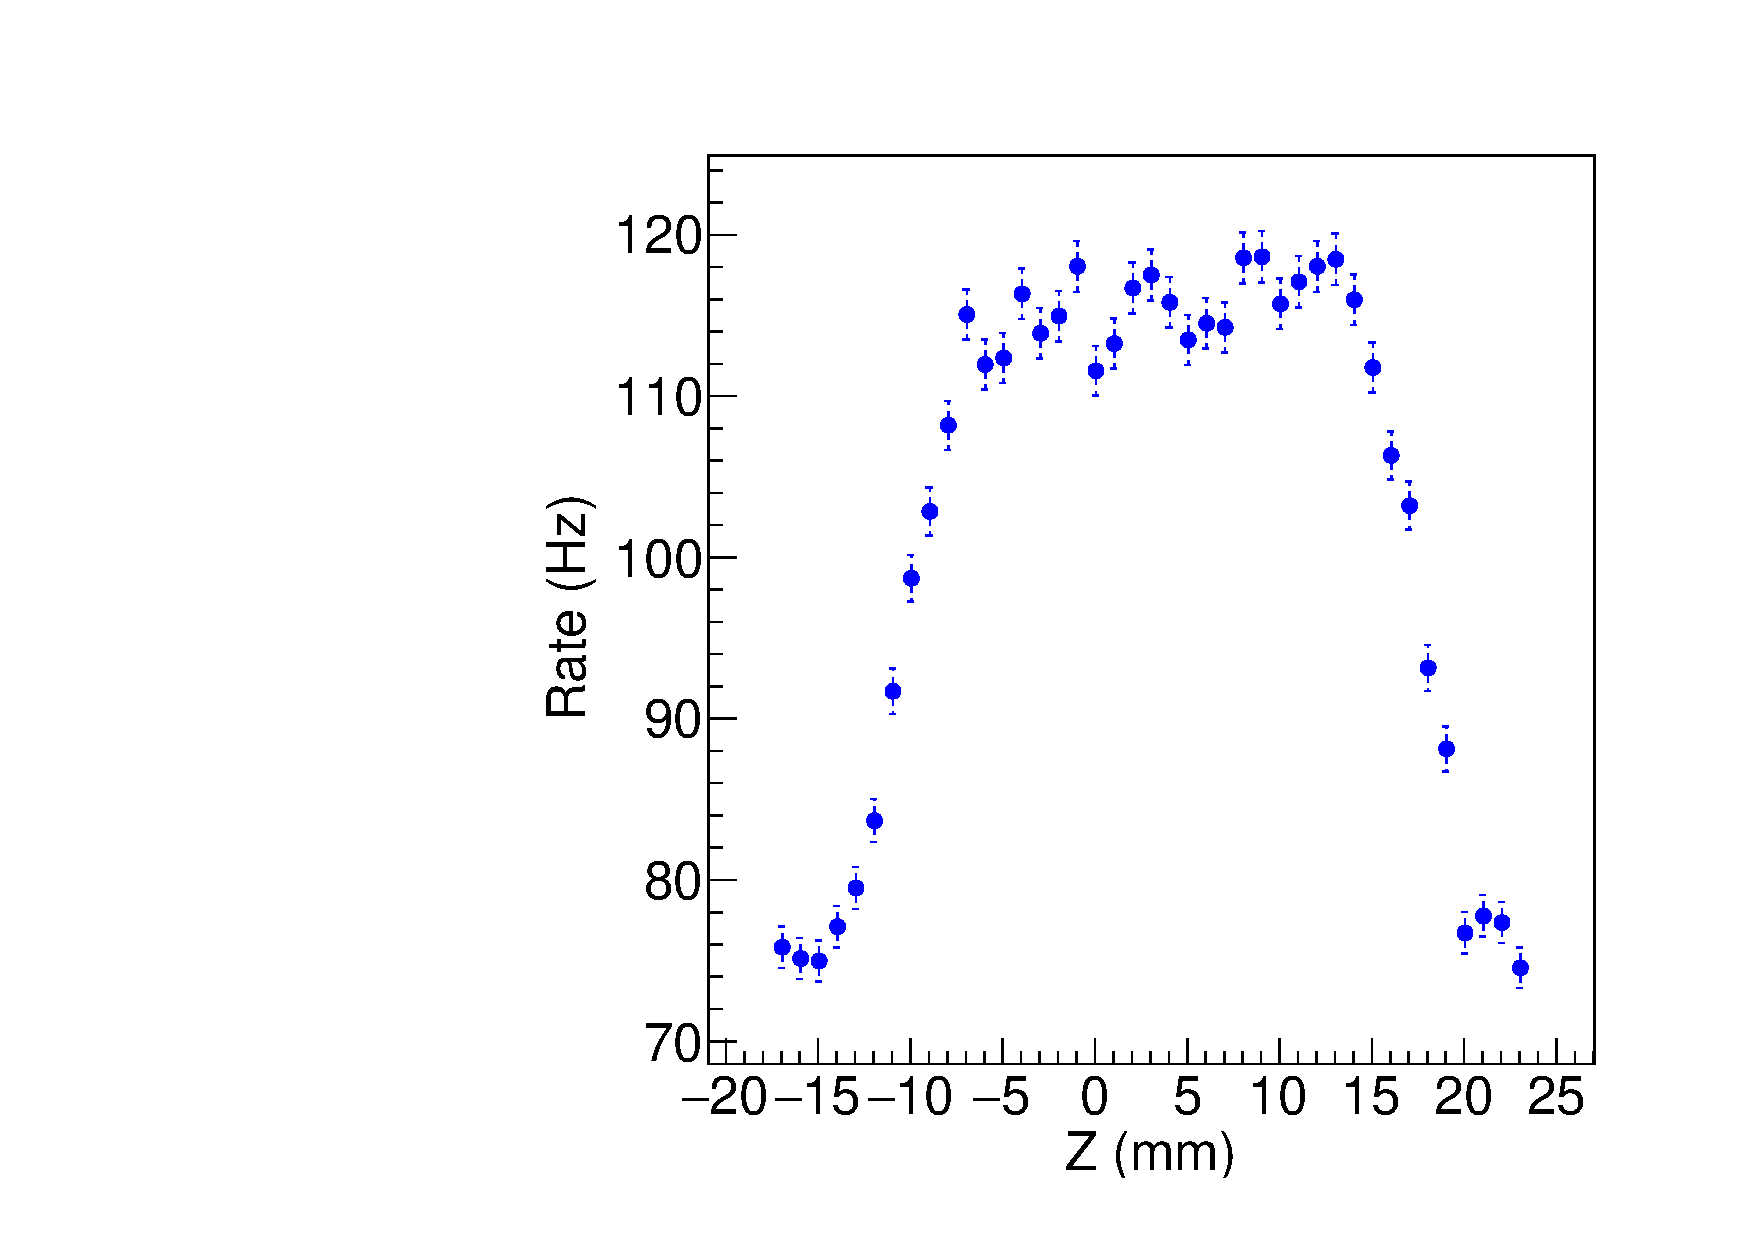
\includegraphics[width=4cm]{plots/xray_lyso3_jun5.pdf}
\caption{Beam profiles in the LYSO scintillator placed on the outer
  wall of COBRA magnet.}
\label{fig:beamprofile}
\end{figure}  

\begin{figure}[]
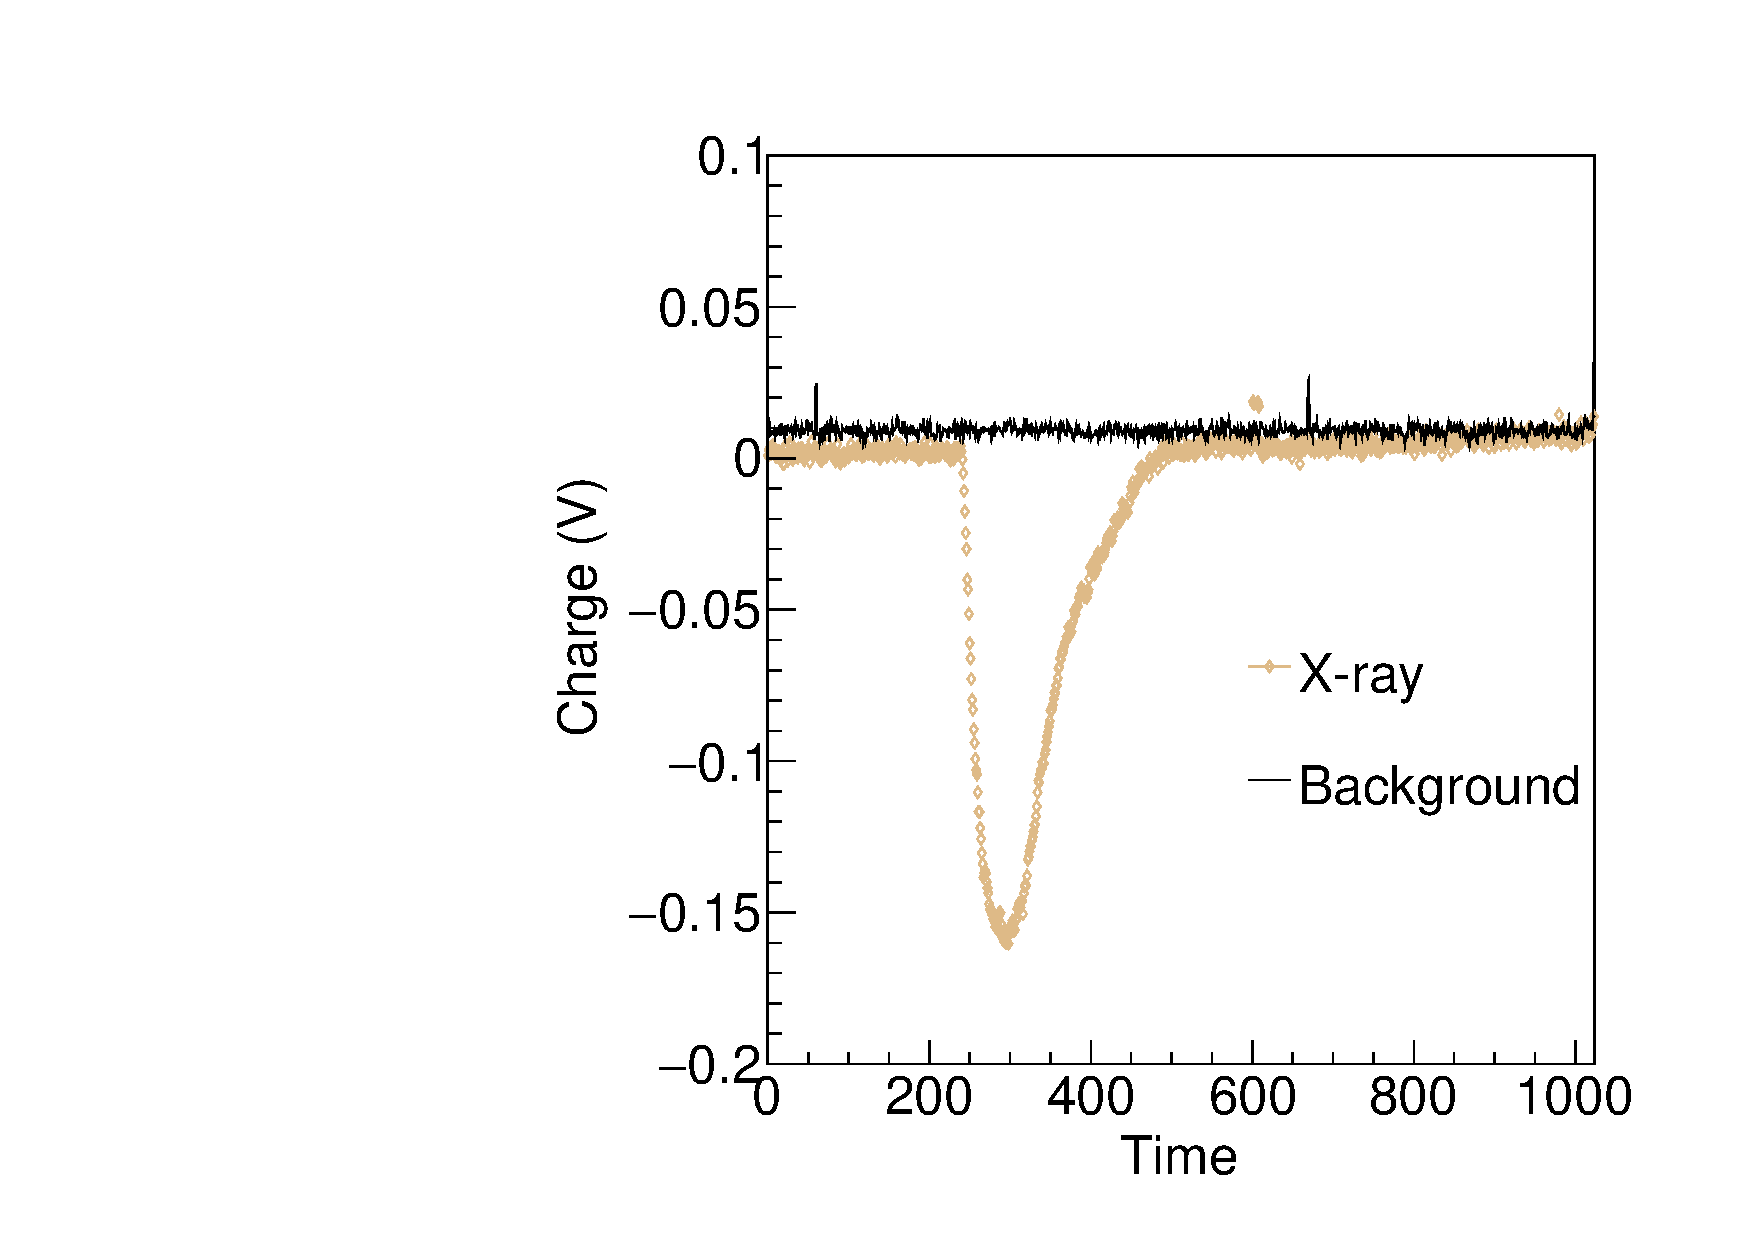
\includegraphics[width=4cm]{plots/mppc1824_waveforms.pdf}
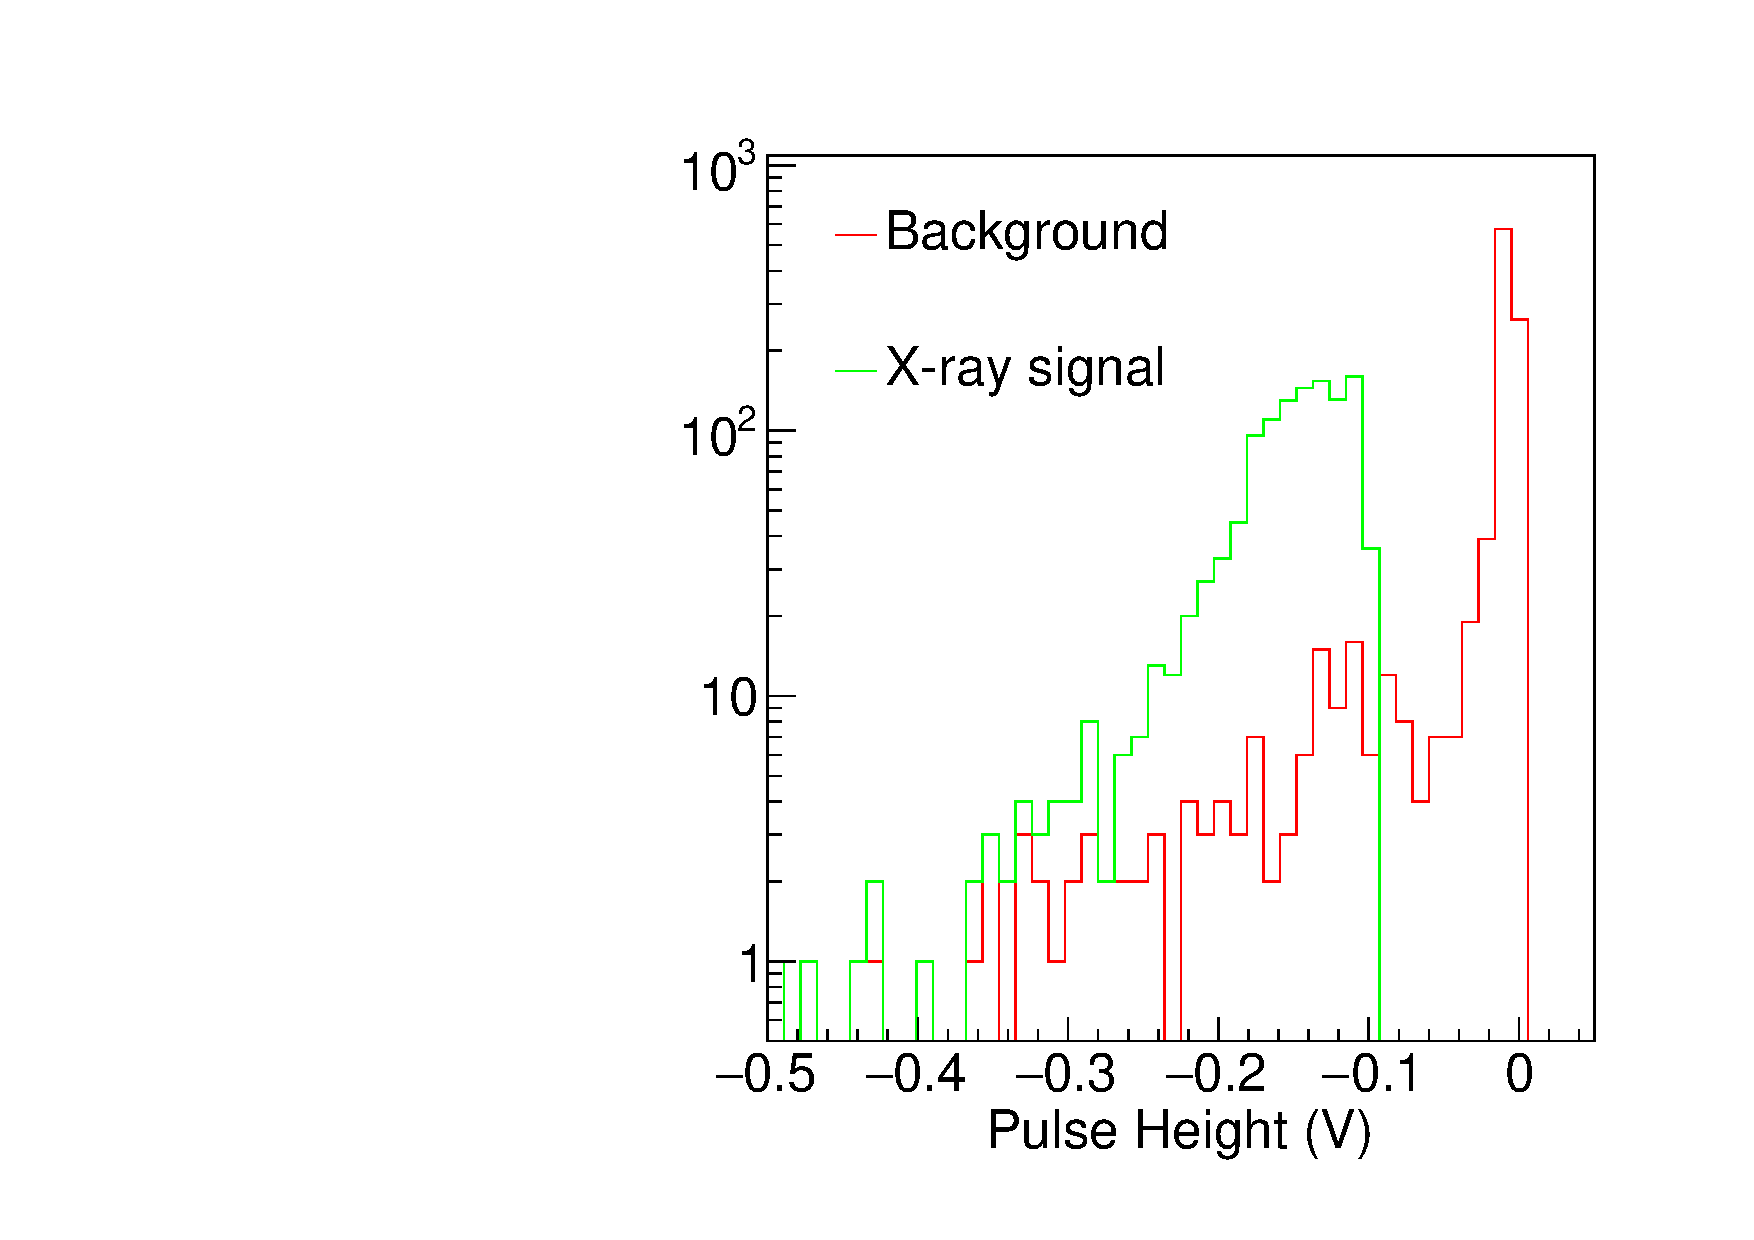
\includegraphics[width=4cm]{plots/pulseheight}
\caption{Recorded waveform and pulse-height data in MPPC channel
  1824.}
\label{fig:pulseheight}
\end{figure}  


\subsection{X-ray device}
The apparatus consists of linear and rotation stages, quadrant photodiode
(QPD), optical laser, camera and bubble-level. A Raspberry Pi device
performs i/o operation with the motion controllers of the motion
stages, and transfers the readout data from the controllers, the QPD
and the camera to the MEG DAQ system.  A software patch was written to
enable the existing MIDAS software framework used for MEG DAQ
operations to communicate with the Raspberry Pi over Gigabit Ethernet.
Downstream processing and analysis is handled by the DAQ system.
 

